\documentclass[11pt, titlepage]{article}

\usepackage{ae, lmodern} % police vectorielle
\usepackage[french]{babel}
\usepackage[utf8]{inputenc}
\usepackage[T1]{fontenc}

\frenchbsetup{og=«,fg=»} % Espaces insécables insérées automatiquement

\pagestyle{headings}

% Packages
\usepackage{graphicx} % Images
\usepackage{hyperref} % Liens cliquables
\usepackage{xcolor}
\usepackage{amssymb}



\setcounter{tocdepth}{2} % Titre de niveau 2 max. (table des matières)

\begin{document}

% 1. PAGE DE TITRE

\begin{titlepage}
\newcommand{\HRule}{\rule{\linewidth}{0.5mm}}
\center

\textsc{\LARGE CY Tech} \\[1cm]


\includegraphics[scale=0.1]{img/cy-tech.png} \\[1cm]

\HRule \\[0.4cm]
{ \huge \bfseries L'euthanasie \\[0.4cm] }
\HRule \\[1.5cm]

{\LARGE Éthique Science et Technique} \\[1cm]

Sonny \bsc{Berthelot}, Alejandro \bsc{Castro}, Marc \bsc{Djolé}, Ewen \bsc{Projac}, Alexandre \bsc{Sauvan} \\[0.2cm]
ING 1, Génie Informatique, Groupe 2 \\[1cm]

13 février 2024 \\ [1cm]

Professeur : Caroline \bsc{Meunier} \\ [1cm]

\end{titlepage}


\newpage

% 2. PAGE DE GARDE
\strut
\thispagestyle{empty} % Retire l'afficahge de la numérotaion de page
\newpage


% 5. SOMMAIRE
\tableofcontents
\newpage


% 6. LISTE DES TABLEAUX ET FIGURES
\listoffigures
\newpage



\section{Introduction}

\subsection{Contexte}

Le morphing est une technique d'animation et d'effets visuels utilisée pour créer une transformation fluide entre deux images ou objets distincts. Ce processus permet de voir une image se métamorphoser progressivement en une autre, en donnant l'illusion que la première se transforme directement en la seconde.

Le morphing est couramment utilisé dans diverses applications, notamment :

\begin{description}
	\item[Cinéma et Télévision] Pour créer des effets spéciaux impressionnants où un personnage ou un objet change de forme de manière spectaculaire ;
	\item[Vidéo musicale] Les clips musicaux utilisent souvent le morphing pour des transitions visuelles créatives et artistiques ;
	\item[Publicité] Pour attirer l'attention et illustrer des transformations de produits ou de services ;
	\item[Logiciels de photographie et d'animation] Offrent des outils de morphing pour les artistes et les animateurs afin de créer des effets visuels captivants.
\end{description}

Un exemple célèbre de morphing dans le cinéma est celui utilisé dans le film "Terminator 2: Judgment Day" (1991), où le personnage du T-1000 change de forme de manière impressionnante. Cette technique a depuis été perfectionnée et est devenue un outil standard dans les effets visuels.


\subsection{Objectif}

L'objectif de ce projet est de réaliser une application de morphing permettant de créer une animation d'une image  \emph{source} à uneimage de  \emph{destination}. Pour ce faire, trois exercices différents sont proposés par le sujet :

\begin{enumerate}
	\item \textbf{Formes simples} : deux polygones de même couleur ;
	\item \textbf{Formes courbées} : deux formes quelconques avec des courbures ;
	\item \textbf{Visages} : deux visages.
\end{enumerate}


\section{Organisation au sein du groupe}

Pour ce projet, nous avons été réparti en groupe de cinq étudiants (GI). Il faut donc s'organiser pour mener à bien le projet pour le 31 mai 2024, date à la quelle la soutenance est prévue.


\subsection{Espace de travail : GitHub}

Ce projet a été l'occasion de découvrir GitHub, un logiciel de partage et de stockage de fichiers optimisé et pensé pour le développement informatique. Il permet de s'échanger des fichiers à distance, voir l'historique des modificaitons et de gérer les conflits en cas de fichiers modifiés par deux presionnes différentes en même temps. C'est pourquoi nous avons choisi cet outil pour nous aider dans la réalistion de notre application de morphing.


\subsection{Répartition des tâches}

Une fois l'environnement de travail pris en main, il nous a fallu nous répartir des tâches à réaliser.

D'abord, il nous fallait nous mettre d'accord sur la méthode à suivre. POur cela, tout le monde à fait des recherches de son côté durant la première semaine en notant les sources consultées qui seront notées dans la bibliographie de ce rapport. Après plusiseurs recherches, nous avons opté pour l'implémentation de la méthode des lignes plutôt que la triangulation de Delaunay.

Globalement, deux groupes se sont formés. Romain et Rubens ce sont occupés de la partie IHM de l'applicaiton ainsi que de la mise en place des contrôleurs. Quant à Rayan et Paul, ils sont focalisés sur la partie back-end du Java avec l'implémentation des algorithmes et des fontions mathématiques nécessaires. Alexandre, a faisait la liaison entre les deux pôles. Néanmoins, quand l'un d'entre nous a une question, il est possible de s'écahnger certaines taĉhes pour s'entraîder. Notre organisaiton est plutôt flexible.


\section{Analyse et conception}

\subsection{Diagramme de cas d'utilisation}


Avant tout projet, un digramme de cas d'utilisation permet de bien se rendre compte des besoins utilisateurs pour ne pas oublier certaines fontionnalités. Ce diagramme est général, il convient donc aux trois exercices du sujet.

\begin{figure}[h]
	\centering
	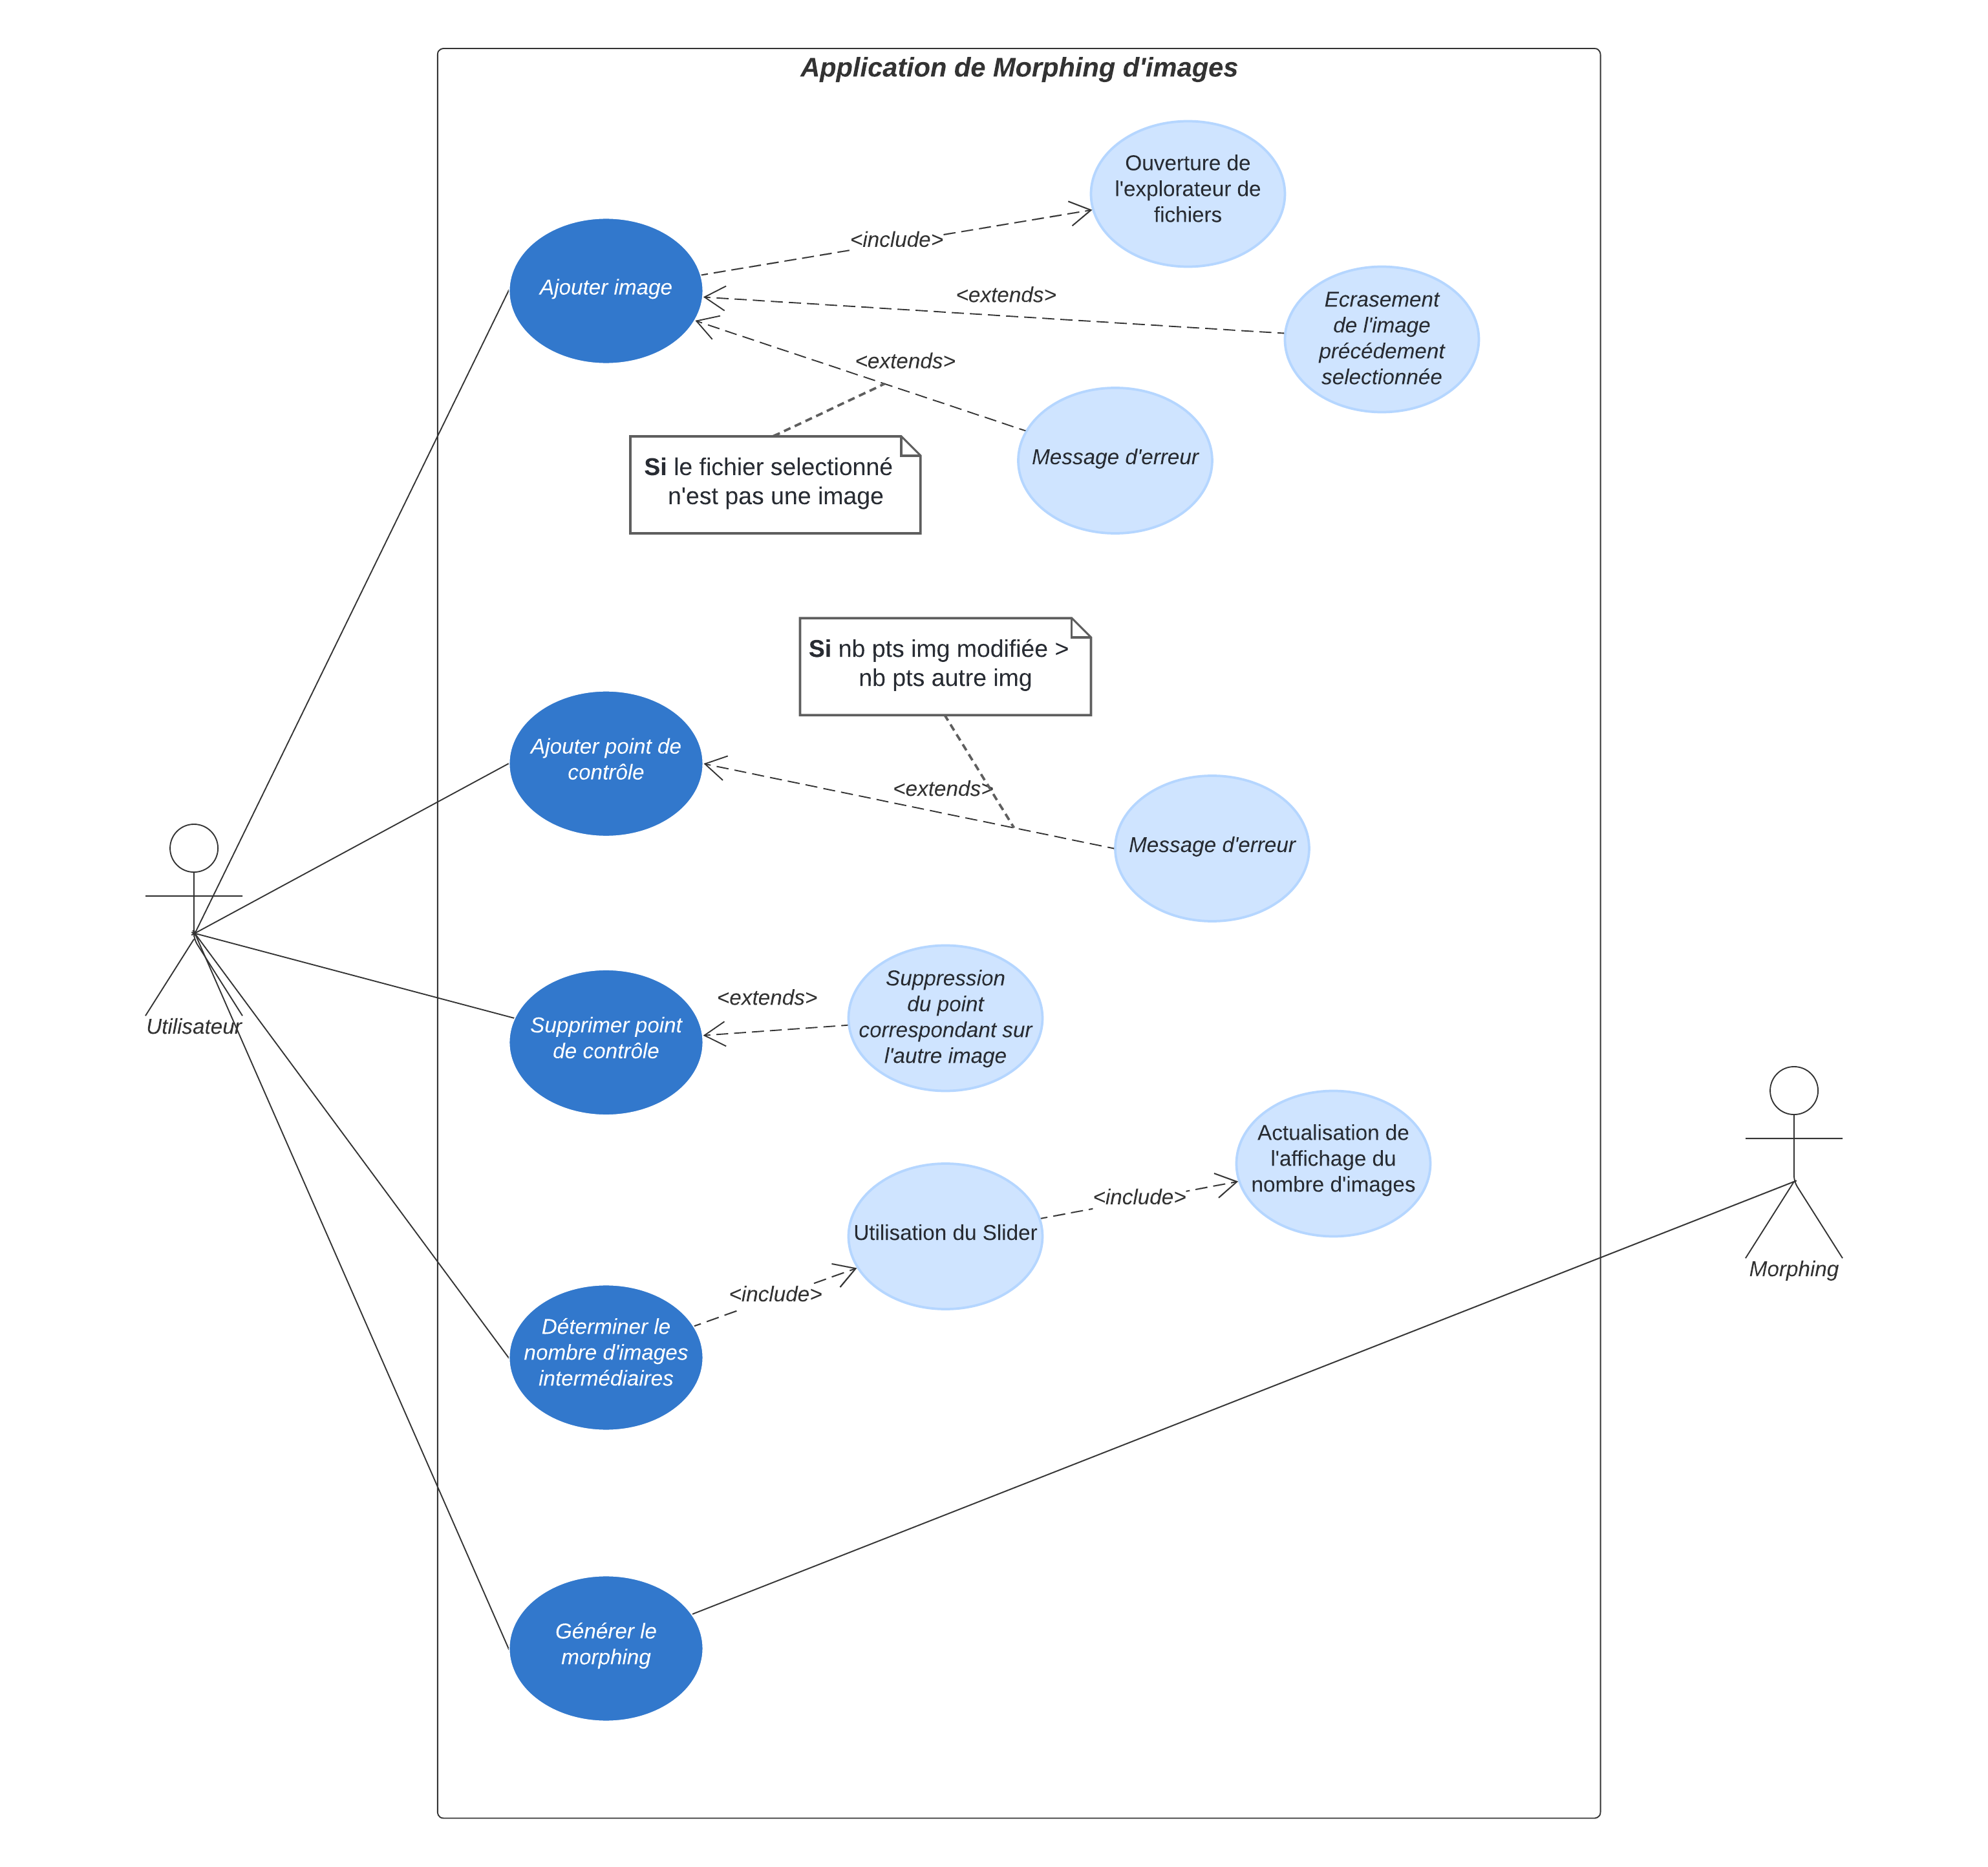
\includegraphics[width=300px]{img/diagramme-utilisation.png}
	\caption{Diagramme de cas d'utilisation}
\end{figure}


\subsection{Diagramme de classe}

Pour pouvoir implémenter nos classes en Java, il est plus que nécessaire de concevoir un diagramme de classe.

\begin{figure}[h]
	\centering
	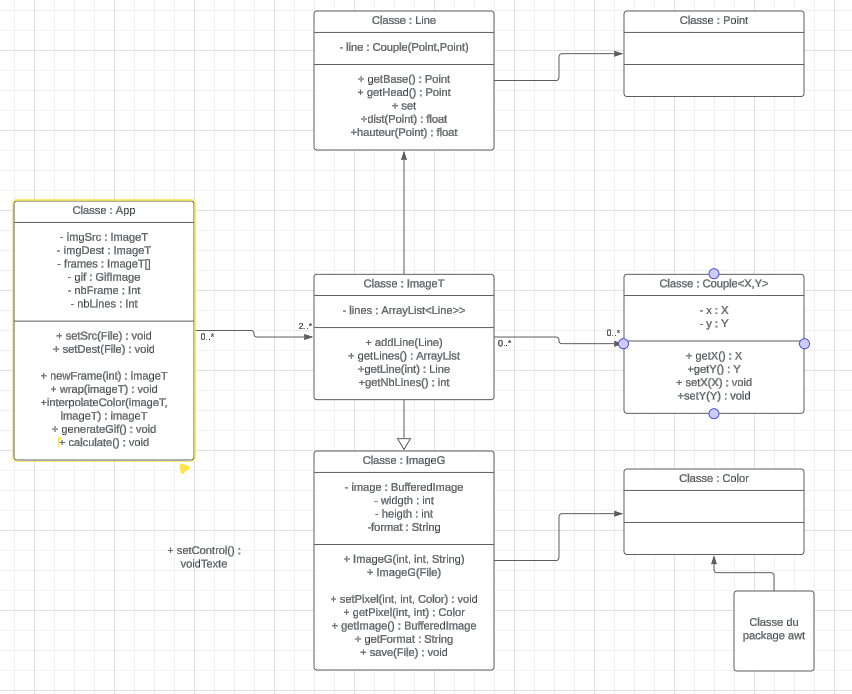
\includegraphics[width=300px]{img/diagramme-classes.png}
	\caption{Diagramme de classe}
\end{figure}


\subsection{Diagramme d'activité}

Un diagramme d'activité est aussi intéressant pour comprendre le focntionnement de l'application.

\begin{figure}[h]
	\centering
	\includegraphics[width=300px]{img/diagramme-activite.png}
	\caption{Diagramme de classe}
\end{figure}


\section{Outils mathématiques}

\subsection{Vecteurs}

\subsection{Projecteurs}

\subsection{L'algorithme de Beier-Neely}


\section{Implémentation en Java}

\subsection{JavaFX (PAC)}

Au niveau de la partie JavaFx nous avons décidé de partir sur une première scène de menu qui nous permet de choisir le type de morphing voulu. Nous avons trois options. Tout d’abord le morphing de formes unies simples. Ensuite le morphing de formes unies arrondies. Enfin la troisième option, le morphing d’images.

Lorsque l’on clique sur l’un des trois boutons, cela quitte la page du menu et ouvre la fenêtre correspondante au morphing souhaité. Par la suite, nous avons opté pour diviser la fenêtre en trois parties. Une à gauche de l’écran, une autre au centre de l’écran et la dernière à droite de l’écran. Dans la partie gauche, nous avons créé un bouton pour ajouter une image dans le carré que l’on a créé dans la partie javaFx. Cette image correspond à l’image de départ. Nous avons fait la même chose à droite mais cette fois-ci l’image correspond à l’image d’arrivée. En revanche, au milieu de l’écran nous avons opté pour un slider qui permet de choisir le nombre d’images intermédiaires à créer pour effectuer le morphing ainsi que du bouton “Morphing” qui permet la création du gif.

Ajoutons également que, quand il y a une photo à droite et à gauche (image de départ et d’arrivée) l’utilisateur peut ajouter des points de contrôles à gauche et à droite. Pour un morphing simple, l’utilisateur ajoute des points sur les images alors que pour un morphing d’images, l’utilisateur ajoute deux points sur une image afin de former une ligne. Il faut noter qu’il faut intervertir l’ajout de point sur les deux images. C'est-à-dire un point à gauche puis un point à droite. Et pour le morphing d’images c’est une ligne à gauche (deux points) puis une ligne à droite (deux points). Tant qu’il n’y a pas le même nombre de points de chaque côté, on ne peut avoir un côté avec plus de points que l’autre. 

Ensuite, toujours dans la partie JavaFx, nous avons opté pour utiliser la méthode PAC (Présentation, Abstraction, Control). La partie présentation est représentée par tout ce qui est le visuel du JavaFx. La partie abstraction représente toute la partie java, c'est-à-dire tout le code, fonctions afin de réaliser un morphing. Finalement, la partie contrôle représente tous les contrôleurs. Il faut un contrôleur pour chaque boutons, sliders, images, points de contrôle. Les contrôleurs font le lien entre la partie java et la partie JavaFx. Nous avons choisie de partir la dessus car cette méthode nous offre de nombreux avantages comme :



\begin{itemize}
	\item Lorsque l’on change quelque chose dans le programme (par exemple dans notre projet, l’image de départ ou le nombre d’images intermédiaires) tous les objets qui ont besoin de ceci seront automatiquement modifiés.
	\item Les objets qui produisent des données  et les objets qui utilisent ces données (les observateurs) sont indépendants. On peut changer l'un sans affecter l'autre. Cela rend le code plus modulaire.
\end{itemize}




\subsection{Librairies}

Nous avons utilisé un certain nombre de librairies afin de réaliser ce projet. Tout d’abord, nous avons utilisé toutes les librairies JavaFx vues et utilisées lors des TD de Java puis nous avons ajouté une autre librairie afin de réaliser le Gif. Les imports réalisés pour obtenir un Gif sont : 

\begin{itemize}
	\item import com.quareup.gifencoder.GifEncoder ;
	\item import com.squareup.gifencoder.ImageOptions.
\end{itemize}


Nous avons également importé les librairies java.io qui permettent de gérer des erreurs.

Ensuite, pour tous les contrôleurs, nous avons importé java.util.Observable ainsi que java.util.Observer.

Pour toute la partie JavaFx, afin de pouvoir avoir des boutons, sliders, labels, des images, ou encore pouvoir cliquer sur un canvas pour afficher des points de contrôles et bien plus, nous avons ajouté toutes les librairies suivantes :


\begin{itemize}
	\item import javafx.embed.swing.SwingFXUtils ;
	\item import javafx.scene.image.Image ;
	\item import javafx.scene.image.ImageView ;
	\item import javafx.application.Application ;
	\item import javafx.geometry.Insets ;
	\item import javafx.geometry.Pos ;
	\item import javafx.scene.Scene ;
	\item import javafx.scene.control.Button ;
	\item import javafx.scene.control.Label ;
	\item import javafx.scene.layout.* ;
	\item import javafx.scene.paint.Color;
	\item import javafx.stage.Stage ;
	\item import javafx.embed.swing.SwingFXUtils ;
	\item import javafx.scene.canvas.Canvas ;
	\item import javafx.scene.canvas.GraphicsContext ;
	\item import javafx.scene.control.Slider ;
	\item import javafx.scene.shape.Rectangle ;
	\item import javafx.scene.text.Text ;
	\item import javafx.stage.Stage.
\end{itemize}



\subsection{Tests unitaires}

\subsection{Bonus : CSS}

Nous avons créé un fichier CSS afin de rendre plus esthétique notre projet. Dans ce fichier, nous avons modifié la couleur de l'arrière-plan de chaque scène. Nous avons également modifier l'apparence des boutons se trouvant dans chaque scène.

\section{Résultat et discussion}

\subsection{Résultats obtenus}

Ainsi, après avoir 

\subsection{Validation des résultats}


\section{Bilan personnel}

Ainsi, après avoir longuement



\bibliographystyle{abbrv}
\bibliography{biblio}



\end{document}
